%-------------------------------------------------------------------------------
\chapter{Experimental Results}
\label{ch.results}
%-------------------------------------------------------------------------------
%\cite{FastMPC}
%\cite{BartlettASvsIP}
%\cite{FerreauASWarm}
%\cite{RaoIPMPC}

This chapter describes the results of the experiments, which were conducted on 
a robot and in a simulation on a personal computer. The experiments on a robot
were performed in order to evaluate and tune the control scheme as a whole.
The comparison of the active set and logarithmic barrier solvers was also
performed in simulation, since there are too many factors that can affect 
the performance on a robot, and it is rather difficult to apply disturbances to 
a robot in a repeatable manner. Note that even in the simulation it is necessary
to check the feasibility of the generated \ac{CoM} trajectory using the inverse
kinematics module. 

The results of the tests presented in this chapter were obtained during a straight 
walk. However, the walking module can realize more complex patterns, for example,
circular walk\footnote{Video recordings of walk patterns realized by our control
module can be accessed at \url{http://www.youtube.com/playlist?list=PL93B16B2910EC7F3D&feature=plcp}}.



%%%%%%%%%%%%%%%%%%%%%%%%%%%%%%%%%%%%%%%%%%%%%%%%%%%%%%%%%%%%%%%%%%%%%%%%%%%%%%%%
%%%%%%%%%%%%%%%%%%%%%%%%%%%%%%%%%%%%%%%%%%%%%%%%%%%%%%%%%%%%%%%%%%%%%%%%%%%%%%%%
%%%%%%%%%%%%%%%%%%%%%%%%%%%%%%%%%%%%%%%%%%%%%%%%%%%%%%%%%%%%%%%%%%%%%%%%%%%%%%%%
\section{Parameters of the Walk and Quadratic Problem}\label{sec.parameters}
The walk is affected by a number of parameters. Some of them were preset, while
others were tuned during experiments on a robot. 

The step height and length were set beforehand. The height of the step is $2$ 
centimeter. The step length is controlled by a parameter, which specifies the 
displacement of a footstep with respect to the previous footstep along the $x$ 
axis. This parameter is equal to $4$ centimeter, hence, the full step length
is $8$ centimeter. 

The parameters of Bezier curves that are used to generate foot trajectories were
found using trial and error approach. The trajectory is shown in \cref{fig.foottraj}.

The length of one \ac{SS} phase is set to $400$ millisecond. The \ac{DS} phase
takes $120$ millisecond and is approximated by $3$ ``fake'' \ac{DS} with rectangular
constraints as described in \cref{sec.ds_constraints}.

The preview window includes $40$ sampling intervals. The first two sampling
intervals are set to $20$ millisecond, since we use the first two states from
the solution of \ac{MPCWMG} (see \cref{sec.mpc_delay} for more information).
The default time for the remaining sampling intervals is $40$ millisecond 
in order to obtain a longer preview window as explained in \cref{sec.timevarsys}.
However, sometimes it is not possible to set all remaining intervals to $40$
millisecond and one of them must be also set to $20$ millisecond. For example,
if one iteration of the control loop is spent in \ac{SS}, the remaining time in
this \ac{SS} is $380$ millisecond, which cannot be divided into intervals of $40$
millisecond. Thus, the total length of the preview window is $2*20 + 38*40 = 1560$ 
or $2*20 + 37*40 + 20 = 1540$ millisecond. 

It is possible to increase the default length of a preview interval, but it has 
negative effects on the gait. Also, the length of all sampling intervals in the
preview window can be set to $20$ millisecond. In this case if the number of 
sampling intervals is not changed, the length of a preview window is significantly 
shorter and a robot does not compensate for external disturbances as well. On the 
other hand, if the number of sampling intervals is increased, a solution of a 
bigger \ac{QP} problem takes more time.

The parameter $\mu_{ik}$, which penalizes the difference with the reference joint
angles in the inverse kinematics \ac{QP} (\cref{sec.ik_alg}), is set to $1.2$.

The gain and threshold for error feedback of \ac{CoM} position are set to $0.3$ 
and $4$ millimeters. The purpose of these parameters is described in 
\cref{sec.err_feedback}. If the threshold is high, the compensation for external
disturbances is not sufficient. 

The solutions of \ac{MPCWMG} are affected by four gains. The first one $\alpha_g$ 
penalizes the difference between the computed \ac{ZMP} trajectory and reference 
\ac{ZMP} points. The last three $\beta_g, \gamma_g, \eta_g$ penalize the absolute
values of velocity, acceleration, and jerk of the \ac{CoM}. It was observed, that 
$\alpha_g$ is the most important. The values of the gains are $\alpha_g = 8000$,
$\beta_g = \gamma_g = \eta_g = 1$. If $\alpha_g$ is set to a smaller value, the 
threshold for \ac{CoM} error feedback must be increased to avoid generation of 
infeasible \ac{CoM} trajectories. 



%%%%%%%%%%%%%%%%%%%%%%%%%%%%%%%%%%%%%%%%%%%%%%%%%%%%%%%%%%%%%%%%%%%%%%%%%%%%%%%%
%%%%%%%%%%%%%%%%%%%%%%%%%%%%%%%%%%%%%%%%%%%%%%%%%%%%%%%%%%%%%%%%%%%%%%%%%%%%%%%%
%%%%%%%%%%%%%%%%%%%%%%%%%%%%%%%%%%%%%%%%%%%%%%%%%%%%%%%%%%%%%%%%%%%%%%%%%%%%%%%%
\section{Experiments on a Robot}
The purpose of the experiments conducted on a Nao robot was to evaluate quality
of the produced gait, compare the two developed \ac{MPCWMG} solvers, and identify
potential improvements of the control scheme.

Initial tuning of the parameters of the walking module was performed using the active
set method. Then the parameters of the logarithmic barrier method were found. The 
approximate solution of the \ac{QP} by logarithmic barrier method does not have
negative effects on the gait (see \cref{fig.com_xy,fig.com_error}).

\begin{figure}[!ht]
    \centering
    \subfigure[\acs{MPCWMG} is solved using the active set method]{
    \includegraphics[scale=0.5]{Figures/as_com_xy.eps}}
    \subfigure[\acs{MPCWMG} is solved using the logarithmic barrier method]{
    \includegraphics[scale=0.5]{Figures/ip_com_xy.eps}}
\caption[Footsteps and projection of {\bf CoM} trajectory to $x\mbox{-}y$ plane]{The 
footsteps and projection of \acs{CoM} to $x\mbox{-}y$ plane. The data is gathered 
during execution of a walking module on a robot. Red and black rectangles show 
positions of the footsteps. \ac{CoM} trajectory generated by the solver is 
represented by the blue curve. The red line shows the measured position of 
\ac{CoM}.}
\label{fig.com_xy}
\end{figure}

During the straight walk the active set method does not deactivate constraints,
the maximal number of added constraints is $7$. In the initial and final double 
supports constraints are not added, during the walk the number of activated 
constraints is usually 6 or 7. The parameters of the logarithmic barrier method 
were selected in such a way that it makes only one iteration of the external 
loop, then the number of internal loops was limited to $3$.

\begin{table}
\begin{center}
\begin{tabular}{c|p{1.5cm}|p{2.5cm}||p{1.5cm}|p{2.5cm}}
            & \multicolumn{2}{c||}{Total time (second)}  & \multicolumn{2}{c}{Solution of the \acs{QP} (second)}\\
\hline
            & Active set method & Logarithmic barrier method & Active set method & Logarithmic barrier method \\
\hline
    minimal & $0.001867$  &   $0.004108$                    & $0.000490$  &   $0.002569$                    \\
    mean    & $0.003071$  &   $0.004834$                    & $0.001259$  &   $0.003016$                    \\
    maximal & $0.004650$  &   $0.006012$                    & $0.002782$  &   $0.004126$                    \\
\end{tabular}
\caption[Execution time of the control loop]{
The amount of time spent in one iteration of the control loop and fraction of this time consumed by the solvers.}
\label{tbl.time}
\end{center}
\end{table}

\begin{figure}[ht]
    \centerline{%
    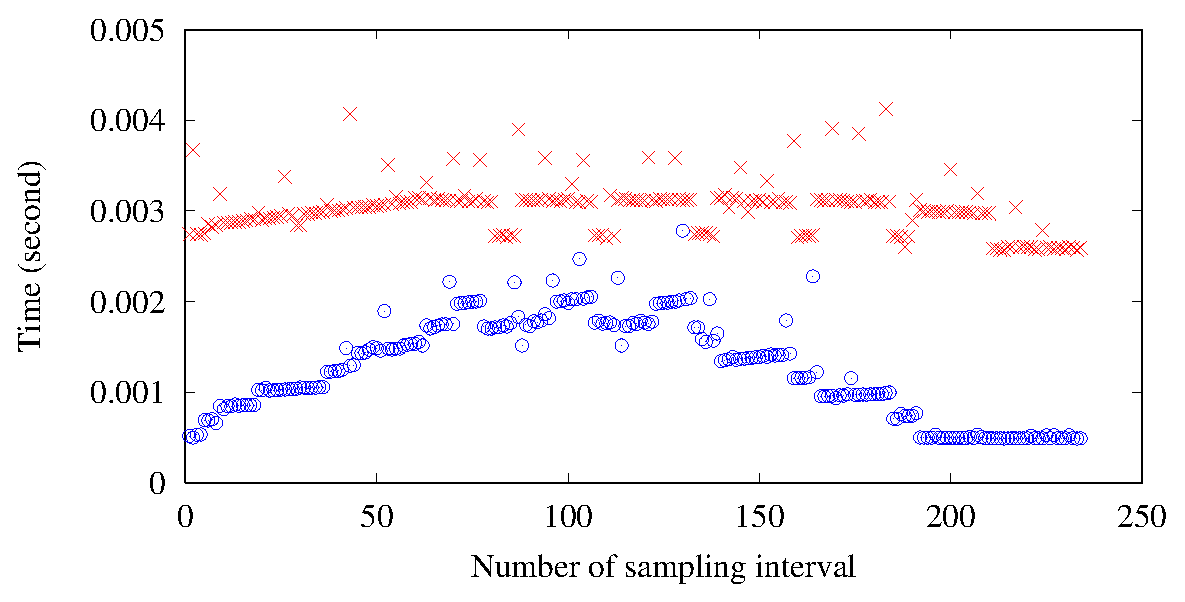
\includegraphics[scale=0.5]{Figures/qp_time.eps}}
    \caption[Execution time of the solvers]{Execution time of the solvers on a robot during
    a straight walk. The red crosses show execution time of the logarithmic barrier method,
    the blue circles -- the active set method.}
    \label{fig.qp_time}
\end{figure}

Measurements of the execution time are presented in \cref{tbl.time} and in 
\cref{fig.qp_time}. The total execution time includes logging, which takes about 
$0.0005$ second, solution of the \ac{MPCWMG} problem, and solution of two inverse 
kinematics problems. The solution of one inverse kinematics problem takes from 
$1$ to $4$ iterations, in $80$\% of cases the number of iterations is not bigger 
than $2$.

\begin{figure}[!ht]
    \centering
%\begin{minipage}[t]{0.48\linewidth}
    \subfigure[Trajectory of the left foot]{
    \includegraphics[scale=0.5]{Figures/left_foot_traj.eps}}
%\end{minipage}
%\hspace{\fill}
%\begin{minipage}[t]{0.48\linewidth}
    \subfigure[Trajectory of the right foot]{
    \includegraphics[scale=0.5]{Figures/right_foot_traj.eps}}
%\end{minipage}
\caption[Foot trajectory tracking]{Tracking of the foot trajectories in $x\mbox{-}z$
plane. The blue line is the trajectory generated using Bezier curve, the red one 
shows the position of the foot computed by forward kinematics function based on the 
measured joint angles.}
\label{fig.robot_foottraj}
\end{figure}

The generated foot trajectories are not followed precisely, due to the action 
of gravity on the swing foot, see \cref{fig.robot_foottraj}. Note that
the right foot does not track the desired trajectory as well as the left.
This effect persists, if the walk is started from different leg. One of the
possible reasons is a flaw of the hardware of the robot, which was used for tests. 

\begin{figure}[ht]
    \centerline{%
    \includegraphics[scale=0.5]{Figures/hiproll.eps}}
    \caption[Joint trajectory tracking]{Tracking of the right hip roll joint trajectory
    produced by the inverse kinematics module. The blue curve is the generated trajectory,
    while the red one shows the measured joint angle.}
    \label{fig.hiproll}
\end{figure}

There is also an error in tracking of joint trajectories, an example is given in
\cref{fig.hiproll}. Several factors cause this error: action of the gravity, 
infeasible joint velocities, and the delay in sensor readings. It is desirable
to account for some of these factors to improve the performance of the walking
module.

\begin{figure}[!ht]
    \centering
%\begin{minipage}[t]{0.48\linewidth}
    \subfigure[Projection of {\bf CoM} trajectory to $x\mbox{-}z$ plane]{
    \includegraphics[scale=0.5]{Figures/as_com_xz.eps}}
%\end{minipage}
%\hspace{\fill}
%\begin{minipage}[t]{0.48\linewidth}
    \subfigure[Projection of {\bf CoM} trajectory to $y\mbox{-}z$ plane]{
    \includegraphics[scale=0.5]{Figures/as_com_yz.eps}}
%\end{minipage}
\caption[Projections of {\bf CoM} trajectory to $x\mbox{-}z$ and $y\mbox{-}z$ planes]{
Projections of \acs{CoM} trajectory generated using the active set method to $x\mbox{-}z$ 
and $y\mbox{-}z$ planes. The data is gathered during execution of a walking module on 
a robot. The reference height of \ac{CoM}, which is always constant, is represented by 
the blue line. The red curve shows the measured position of \ac{CoM}.}
\label{fig.com_xyz}
\end{figure}

\begin{figure}[!ht]
    \centering
%\begin{minipage}[t]{0.48\linewidth}
    \subfigure[\acs{MPCWMG} is solved using the active set method]{
    \includegraphics[scale=0.5]{Figures/as_com_error.eps}}
%\end{minipage}
%\hspace{\fill}
%\begin{minipage}[t]{0.48\linewidth}
    \subfigure[\acs{MPCWMG} is solved using the logarithmic barrier method]{
    \includegraphics[scale=0.5]{Figures/ip_com_error.eps}}
%\end{minipage}
\caption[Error in {\bf CoM} position]{Error in \ac{CoM} position. Blue, red, 
and black lines correspond to error along $x$, $y$, and $z$ axes, respectively.}
\label{fig.com_error}
\end{figure}

Due to the errors in tracking of foot and joint trajectories and, probably,
other factors, a significant error in \ac{CoM} appears (see 
\cref{fig.com_xy,fig.com_xyz,fig.com_error}). The performance heavily depends 
on the error feedback. If the error feedback is disabled by setting the 
respective gain to zero, the robot starts to wobble after a few steps and 
soon falls.

It was mentioned in \cref{sec.err_feedback}, that there is a second type of 
error feedback, which corrects the positions of footsteps. The result of this
feedback can be clearly seen in \cref{fig.com_xy}, when compared to the 
footsteps obtained in simulation that are shown in \cref{fig.footsteps}.



%%%%%%%%%%%%%%%%%%%%%%%%%%%%%%%%%%%%%%%%%%%%%%%%%%%%%%%%%%%%%%%%%%%%%%%%%%%%%%%%
%%%%%%%%%%%%%%%%%%%%%%%%%%%%%%%%%%%%%%%%%%%%%%%%%%%%%%%%%%%%%%%%%%%%%%%%%%%%%%%%
%%%%%%%%%%%%%%%%%%%%%%%%%%%%%%%%%%%%%%%%%%%%%%%%%%%%%%%%%%%%%%%%%%%%%%%%%%%%%%%%
\section{Experiments in a Simulation}
One of the goals of the thesis is to compare active set and logarithmic barrier
methods for solution of \ac{MPCWMG}. Comparison of these methods in the presence
of external disturbances on a robot is complicated due to the necessity to apply such
disturbances in a repeatable manner. Hence, some of the tests were performed
during simulation of the walk on a personal computer. The \ac{CoM} trajectories 
were generated with the same parameters as on the robot. The inverse kinematics 
module was adopted to ensure feasibility of these trajectories, since neither 
optimality or stability of \ac{MPCWMG} solutions imply feasibility (see 
\cref{fig.sim_dist}).

The \ac{CoM} trajectories that were obtained in the simulation without any 
disturbances are shown in \cref{fig.sim_nodist}.

\begin{figure}[!ht]
    \centering
%\begin{minipage}[t]{0.48\linewidth}
    \subfigure[Trajectory generated using the active set method]{
    \includegraphics[scale=0.5]{Figures/sim_nodist_as.eps}}
%\end{minipage}
%\hspace{\fill}
%\begin{minipage}[t]{0.48\linewidth}
    \subfigure[Trajectory generated using the logarithmic barrier method]{
    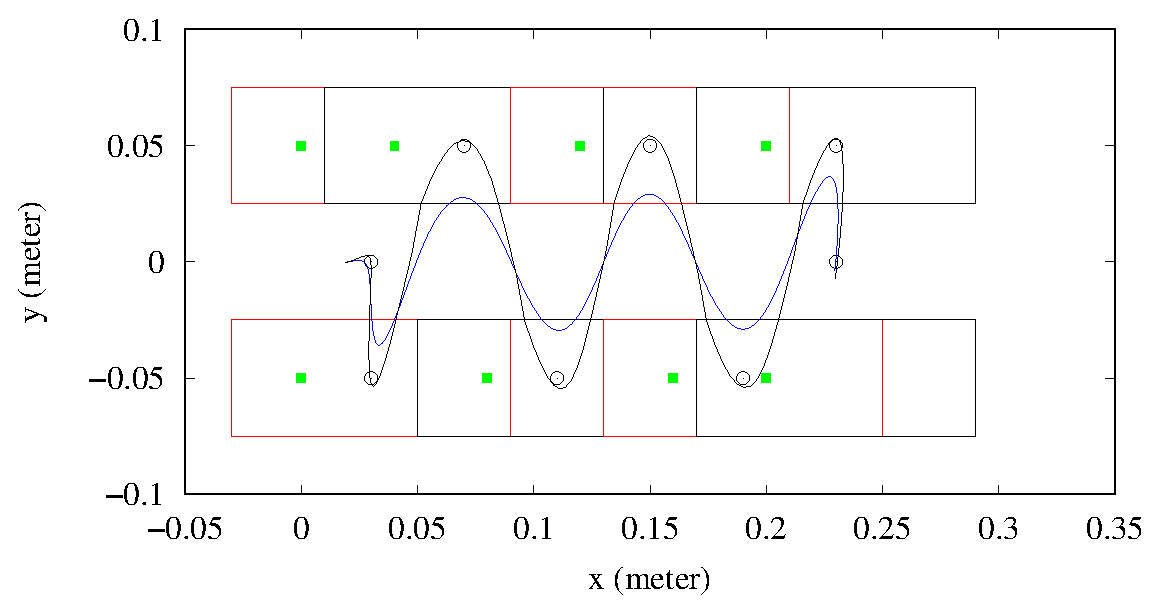
\includegraphics[scale=0.5]{Figures/sim_nodist_ip.eps}}
%\end{minipage}
\caption[Trajectories of {\bf CoM} in a simulation]{Trajectories of {\bf CoM} in a 
simulation. Red and black rectangles represent \ac{SS}, \ac{DS} are omitted. Blue 
and black curves show trajectories of \ac{CoM} and \ac{ZMP}, respectively. Black 
circles stand for reference \ac{ZMP} positions. Green boxes are the footstep 
reference points.}
\label{fig.sim_nodist}
\end{figure}

The disturbances are applied by instantaneous change of the position of \ac{CoM} 
to replicate error feedback on the robot. An example is shown in \cref{fig.sim_dist}. 
During one simulation run the system is disturbed only once. The displacement of
\ac{CoM} is no more than two centimeters along one of the axes in the horizontal
plane. 

It was observed that strong disturbances (more than one centimeter) often lead to 
instability of the \ac{MPCWMG}, when the \ac{CoM} trajectory diverges. 

\begin{figure}[!ht]
    \centering
%\begin{minipage}[t]{0.48\linewidth}
    \subfigure[Trajectory generated using the active set method]{
    \includegraphics[scale=0.5]{Figures/sim_infeas_as.eps}}
%\end{minipage}
%\hspace{\fill}
%\begin{minipage}[t]{0.48\linewidth}
    \subfigure[Trajectory generated using the logarithmic barrier method]{
    \includegraphics[scale=0.5]{Figures/sim_infeas_ip.eps}}
%\end{minipage}
\caption[Trajectories of {\bf CoM} in the presence of disturbance]{Trajectories of 
{\bf CoM} in the presence of disturbance. Red and black rectangles represent \ac{SS}, 
\ac{DS} are omitted. Blue and black curves show trajectories of \ac{CoM} and \ac{ZMP}, 
respectively. Black circles stand for reference \ac{ZMP} positions. Green boxes are 
the footstep reference points. The red stars indicate infeasible \ac{CoM} positions.}
\label{fig.sim_dist}
\end{figure}

The disturbances have a strong effect on the performance of the active set method, since
the number of constraints at the optimal point is often higher. In some situations the size
of the active set reaches $40$, which makes the solution computationally infeasible on a 
robot. In order to enforce the time limits, the deactivation of constraints can be disabled 
and the maximal number of activated constraints can be fixed. If the limit on the number 
of the activated constraints is relatively high (bigger than $20$), the approximate solution 
is often admissible. However, strict limits, as well as disabled deactivation of constraints
may lead to instability.

\begin{figure}[ht]
    \centerline{%
    \includegraphics[scale=0.5]{Figures/obj_asip.eps}}
    \caption[The decrease rate of objective function]{The decrease rate of objective 
    function. The values produced using active set and logarithmic barrier method 
    are represented by the blue and red lines, respectively.}
    \label{fig.obj_asip}
\end{figure}

The \ac{MPCWMG} may also become unstable, if there are no disturbances, but a rather 
strict limit on the number of active constraints is imposed. The properly tuned
logarithmic barrier method can be safer in this case, since it results in higher 
decrease rate of the value of the objective function (see \cref{fig.obj_asip})
in the number of iterations.
